\documentclass[notes]{subfiles}
\begin{document}
	\addcontentsline{toc}{section}{3.3 - Differentiation Rules}
	\refstepcounter{section}
	\fancyhead[RO,LE]{\bfseries \nameref{cs33}} 
	\fancyhead[LO,RE]{\bfseries \small \currentname}
	\fancyfoot[C]{{}}
	\fancyfoot[LO,RE]{\large \thepage}	%Footer on Right \thepage is pagenumber
	\fancyfoot[RO,LE]{\large Chapter 3.3}
	
	
\section*{Differentiation Rules}\label{cs33}
	\subsection*{Before Class}
	\subsubsection*{Constant Functions}
		\begin{ex}
			Use the definition of the derivative to find \(f'(x)\), where \(f(x) = 2\).
		\end{ex}
			\vs{1}
			
		\begin{ex}
			Find the derivative of an arbitrary constant \(c\).
		\end{ex}
			\vs{1}
			
		\begin{thm}[Constant Rule]
			If \(f(x) = c\), \(c\) a constant, then 
			
				\vspace{.25in}
			
		\end{thm}
			\vs{1}
			\newpage
	
	\subsubsection*{Power Functions}	
		\begin{ex}
			Find the derivative of \(f(x) = x\)
		\end{ex}
			\vs{.5}
			
		\begin{ex}
			Find the derivative of \(f(x) = x^2\)
		\end{ex}
			\vs{.75}
			
		\begin{ex}
			Find the derivative of \(f(x) = x^3\)
		\end{ex}
			\vs{1}
		
		\begin{ex}
			Find the derivative of \(f(x) = x^4\)
		\end{ex}	
			\vs{1.5}
			\newpage
			
		\begin{question}
			What is the pattern in these derivatives? Look at the powers...
		\end{question}
			\vs{1}
			
		\begin{thm}[Power Rule]
			If \(f(x) = x^n\), then 
			
				\vspace{.25in}
			
		\end{thm}
			\vs{.25}
			
		\begin{ex}
			Find \(\dfrac{d}{dx}[x^{99}]\)
		\end{ex}
			\vs{1}

	\subsection*{New Derivatives from Old}
		\begin{ex}
			Using definition of the derivative, find the derivative of \(f(x) = 3x^2\)
		\end{ex}
			\vs{1.5}
			\newpage
			
		\begin{ex}
			Using definition of the derivative, find the derivative of \(f(x) = -2x^3\)
		\end{ex}
			\vs{1.5}
			
		\begin{question}
			What relationship do you notice between these derivatives and the coefficients?
		\end{question}
			\vs{1}
			
		\begin{thm}[Constant Multiple Rule]
			If \(c\) is a constant and \(f\) is a differentiable function, then\\[25pt]
			
		\end{thm}
			
		There are three more important rules:
		\begin{thm}[Sum/Difference Rule]
			If \(f\) and \(g\) are differentiable functions, then\\[25pt]
			
		\end{thm}
			\vs{.25}
	
			\newpage
			
		\begin{thm}[Product Rule]
			If \(f\) and \(g\) are both differentiable, then\\[75pt]
			
		\end{thm}
			\vs{.25}
			
		\begin{ex}
			Compute the derivative of \(f(x) = x^3\cdot x^5\)
		\end{ex}
			\vs{1} 

		\begin{thm}[Quotient Rule]
			If \(f\) and \(g\) are both differentiable (with \(g\neq 0\)), then\\[75pt]
			
		\end{thm}
			\vs{.25}

		\begin{ex}
			Compute the derivative of \(g(x) = \dfrac{x}{x+1}\)
		\end{ex}
			\vs{1}
			\newpage
			
	\subsection*{Pre Class Practice}
		\begin{ex}
			Find the derivative of the function \(f(x) = 2^{40}\)
		\end{ex}
			\vs{1}
			
		\begin{ex}
			Find the derivative of the function \(f(t) = 1.4t^5 -2.5t^2 + 6.7\)
		\end{ex}
			\vs{1}
			
		\begin{ex}
			Find the derivative of the function \(B(y) = cy^{-6}\), where \(c\) is an arbitrary constant.
		\end{ex}
			\vs{1}
			
		\begin{ex}
			Find the derivative of the function \(y = \dfrac{x^2+4x+3}{\sqrt{x}}\) two ways: first, by the quotient rule; then, by splitting the fraction, simplifying, and rewriting.
		\end{ex}
			\vs{1}
			\newpage
			
	\subsection*{In Class}
	\subsubsection*{Examples}
		\begin{ex}
			For the following functions, find the derivatives.  Then, find an equation for the tangent line to the function at the given point.
			\begin{enumerate}[(a)]
				\item \(S(p) = \sqrt{p}-p\) at \((9,-6)\)
					\vs{1}
					
			 	\item \(F(r) = \dfrac{5}{r^3}\) at \((-2,-5/8)\)
			 		\vs{1}
			 		
				\item \(A(r) = \pi r^2\) at \((1,\pi)\)
					\vs{1}
			\end{enumerate}
		\end{ex}
		
		\begin{ex}
			Find the derivatives of the following functions.
			\begin{enumerate}[(a)]
				\item \(F(y) = \lrpar{\dfrac{1}{y^2}-\dfrac{3}{y^4}}(y+5y^3)\)
					\vs{1}
					\newpage
					
				\item \(J(v) = (v^3-2v)(v^{-4}+v^{-2})\)
					\vs{1}
					
				\item \(f(x) = \dfrac{1+2x}{3-4x}\)
					\vs{1}
					
				\item \(Y(t)=\dfrac{1}{t^3+2t^2-1}\)
					\vs{1}
					
		 		\item \(h(u) = \dfrac{(u+2)^2}{1-u}\)
		 			\vs{1}
		 			\newpage
		 			
				\item \(f(t) = \dfrac{\sqrt[3]{t}}{t-3}\)
					\vs{1}
					
			\end{enumerate}
		\end{ex}
		
		\begin{ex}
			Let \(f(x) = 2x^3-x^2+1\).  The \emph{normal line} through a point is the line which is perpendicular to the tangent line.
			\begin{enumerate}[(a)]
				\item Find the equation of the tangent line to \(f(x)\) at \((1,2)\).
					\vs{1}
					
				\item Find the equation of the normal line to \(f(x)\) at \((1,2)\).
					\vs{1}
			\end{enumerate}
		\end{ex}
			
		\begin{ex}
			Let \(f(x) = \dfrac{2x}{x+1}\). Find the equation of the tangent line to \(f(x)\) at \((1,1)\).
				\vs{1}

		\end{ex}

		\begin{ex}
			If \(H(x) = xf(x)\), find an expression for \(H'(x)\)
		\end{ex}
			\vs{.75}
			\newpage
			
		\begin{ex}
			Suppose that \(f(5) = 1\), \(f'(5) = 6\), \(g(5) = -3\), and \(g'(5) = 2\).  Find
			\begin{enumerate}[(a)]
				\item \((fg)'(5)\)
					\vs{.5}
					
				\item \((f/g)'(5)\)
					\vs{.5}
					
				\item \((g/f)'(5)\)
					\vs{.5}
					
			\end{enumerate}
		\end{ex}
		
		\begin{ex}
			If \(h(2) = 4\) and \(h'(2) = -3\), find \(\dfrac{d}{dx} \lrpar{\dfrac{h(x)}{x^2}}\bigg\rvert_{x = 2}\)
		\end{ex}
			\vs{1}
		
		\begin{ex}
			If \(f\) and \(g\) are the functions on the graph shown, let \(u(x) = f(x)g(x)\) and \(v(x) = f(x)/g(x)\).  Find \(u'(1)\) and \(v'(5)\).\\
			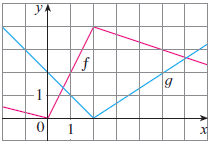
\includegraphics{3.3fig1}
		\end{ex}	
			\vs{.5}
			\newpage
	
	\subsection*{After Class Practice}		
		\begin{ex}
			Suppose that \(f(4) = 2\), \(g(4) = 5\), \(f'(4) = 6\), and \(g'(4) = -3\).  Find \(h'(4)\) if:
			\begin{enumerate}[(a)]
				\item \(h(x) = 3f(x) + 8g(x)\)
					\vs{1}
				
				\item \(h(x) = f(x)g(x)\)
					\vs{1}
					
				\item \(h(x) = \dfrac{f(x)}{g(x)}\)
					\vs{1}
					
				\item \(h(x) = \dfrac{g(x)}{f(x) + g(x)}\)
					\vs{1}
			\end{enumerate}
		\end{ex}
		
		\begin{ex}
			If \(f\) is a differentiable function, find an expression for the derivative of each of the following:
			\begin{enumerate}[(a)]
				\item \(y = x^3f(x)\)
					\vs{1}
					
				\item \(y = \dfrac{f(x)}{x}\)
					\vs{1}
					\newpage
					
				\item \(y = \dfrac{x^2}{f(x)}\)
					\vs{1}
					
				\item \(y = \dfrac{1 + xf(x)}{\sqrt{x}}\)
					\vs{1}
			\end{enumerate}
		\end{ex}
		
		\begin{ex}
			For what values of \(x\) does the graph of \(f(x) = x^3 + 3x^2 + x + 3\) have a horizontal tangent?
		\end{ex}
			\vs{1}
			
		\begin{ex}
			Show that the vertex of any quadratic function occurs at \(x=-\dfrac{b}{2a}\)
		\end{ex}
			\vs{1}
	

\clearpage
\end{document}
